\documentclass[a4paper, 10pt, conference]{ieeeconf}      % Use this line for a4 paper
\IEEEoverridecommandlockouts                              % This command is only needed if 
                                                          % you want to use the \thanks command
\overrideIEEEmargins                                      % Needed to meet printer requirements.
% See the \addtolength command later in the file to balance the column lengths
% on the last page of the document
\usepackage[english]{babel}
\usepackage[utf8]{inputenc}
\usepackage[a4paper]{geometry}
\geometry{top=44mm, bottom=20mm, left=20mm, right=14mm}
\usepackage[pdftex]{graphicx}

\usepackage{amsfonts}
\usepackage{amssymb}
\usepackage{mathrsfs}
\usepackage{amsmath}
%\usepackage{amsthm}
\usepackage{color}

\newtheorem{theorem}{Theorem}
\newcommand{\tr}[1]{\textcolor{red}{#1}}

\title{\LARGE \bf
Dynamic optimisation of resource allocation in microorganisms (extended abstract)
}

\author{Nils Giordano$^{1,2}$, Francis Mairet$^{3}$, Jean-Luc Gouzé$^{3}$, Johannes Geiselmann$^{1,2}$, Hidde de Jong$^{2}$*% <-this % stops a space
\thanks{*Corresponding author: hidde.de-jong@inria.fr}% <-this % stops a space
\thanks{$^{1}$Laboratoire Adaptation et Pathog\'enie des Microorganismes (CNRS UMR 5163),
Universit\'e Joseph Fourier,
La Tronche, France}
\thanks{$^{2}$Inria Grenoble--Rh\^one-Alpes, Montbonnot, 38334 Saint-Ismier Cedex, France}
\thanks{$^{3}$Inria Sophia Antipolis M\'editerran\'ee, 06902 Sophia Antipolis, France}
}


\begin{document}
\maketitle
\thispagestyle{empty}
\pagestyle{empty}
%%%%%%%%%%%%%%%%%%%%%%%%%%%%%%%%%%%%%%%%%%%%%%%%%%%%%%%%%%%%%%%%%%%%%%%%%%%%%%%%
\begin{abstract}

Bacterial growth is a fundamental process in which cells sustain and reproduce themselves from available matter and energy.
Optimisation principles have been widely used to explain and predict the growth behaviour of microorganisms, assumed to be optimized by evolution.
This has given rise, among other things, to bacterial growth laws describing how the abundance of components of the gene expression machinery increases with the growth rate. These studies have mainly focused on the situation where the system is in balanced growth, a steady state in which all cell components grow at the same rate.
Balanced-growth conditions, however, are far from natural growth conditions in which the environment is continually changing.
We focus on the optimal allocation of resources between the gene expression machinery and other subsystems during growth-phase transitions.
We describe an abstract model of the biochemical reaction processes occurring in the cell, based on first principles and articulated around two subsystems: the gene expression machinery and the uptake of nutrients from the environment.
Using this so-called self-replicator model, we investigate the optimal dynamic reallocation of resources following a rapid change in the environment.
We formulate our question as an optimal control problem that can be solved using Pontryagin's maximum principle.
Preliminary results have shown the predominance of bang-singular control of resource allocation following abrupt environmental transitions.
\end{abstract}

% introduction
One of the fundamental properties of life is the maintenance and replication of cells from available matter and energy.
Microorganisms are excellent models for the study of this autopoetic process, as they undergo a strong selective pressure for growth.
Extensive studies in quantitative bacterial physiology have yielded a number of important insights, like the growth-rate dependence of the cell composition (DNA, RNA, protein, ...) and the key role of the gene expression machinery in controlling growth \cite{scott_interdependence_2010,bremer_modulation_1996,maaloe_control_1966}.
This has contributed to the development of empirical bacterial growth laws, reviewed in \cite{scott_bacterial_2011}.

Optimisation theory is important for understanding how growth laws arise from evolution and physical constraints on living matter.
Indeed, it is widely accepted that microorganisms are mostly optimised for growth \cite{dekel_optimality_2005}.
As a consequence, much theoretical work on bacterial growth has been based on optimisation principles, with several successes at the metabolic, genetic or global cell level \cite{edwards_escherichia_2000, molenaar_shifts_2009}.

These studies generally focus on the balanced growth of a bacterial population, that is, a steady state in which all cell components grow at the same rate \cite{neidhardt_physiology_1990}.
Balanced growth is a convenient condition to study growth, since it is experimentally reproducible and leads to mathematically simple models.
However, the constant environmental conditions necessary for balanced growth are easy to simulate in the laboratory, but hard to find in nature \cite{neidhardt_physiology_1990}.
In most situations bacterial cells have to continually adapt their growth rate and their molecular composition, notably the sets of expressed proteins (proteome), to changes in the availability of nutrients and other environmental parameters.

Despite the large amount of work on bacterial growth, as stated in a recent study "little is known about the dynamics of proteome change, e.g., whether bacteria use optimal strategies of gene expression for rapid proteome adjustments..." \cite{pavlov_optimal_2013}.
This study and other recent work \cite{ehrenberg_medium-dependent_2013} have argued that it is important to consider optimisation principles from a dynamic perspective when studying bacterial growth.
In this contribution, we extend the above ideas by focusing on the dynamics of a key proteome component, the gene expression machinery.
More precisely, our aim is to study the optimal allocation of resources to the gene expression machinery and to the uptake of nutrients from the environment during growth-phase transitions, using tools from optimal control theory.

% model description
In order to model bacterial growth and relate it to the environment and the molecular composition of the cell, we use the self-replicator model introduced by Molenaar and colleagues \cite{molenaar_shifts_2009}.
This abstract model, built from first principles, articulates self-replication around the gene expression machinery R and the metabolic machinery M (Figure \ref{fig::selfrep}). While M converts substrate S from the environment into precursors P, R transforms these precursors into macromolecules, including the transporters and enzymes in M and the RNA polymerases and ribosomes in R.
\begin{figure}[htpb]
\centering
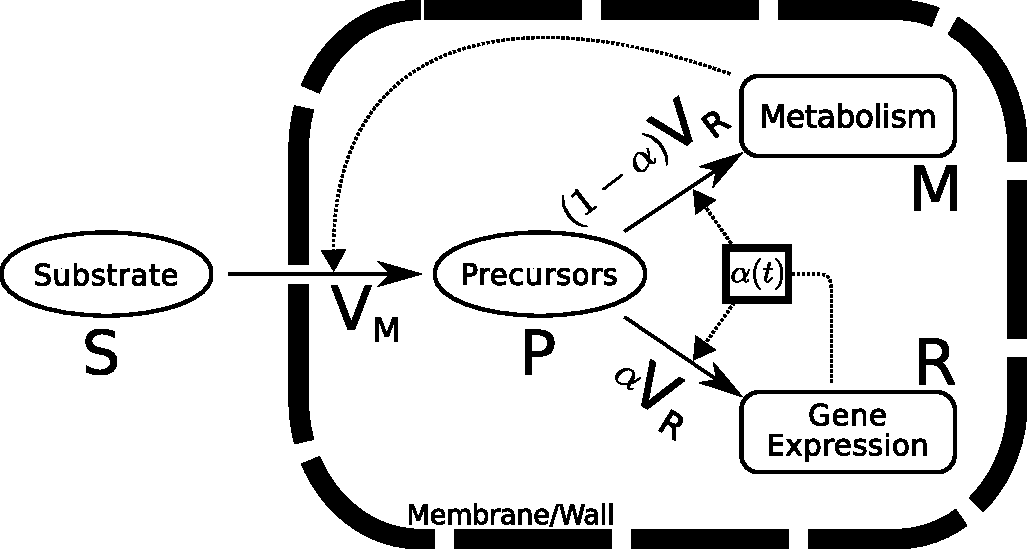
\includegraphics[width=0.45\textwidth]{../../Fig/model_apr2014_baw.pdf}
\caption{\textbf{Self-replicator model.} S, P, M, and R refer to substrate, precursors, metabolic machinery and gene expression machinery, respectively.
$V_M$ and $V_R$ are reaction rates.
$\alpha(t)$ is the gene regulation control variable.
}
\label{fig::selfrep}
\end{figure}

The self-replicator system is described by the following two reactions:
\begin{eqnarray*}
S  &\overset{V_M}{\longrightarrow}& P \\
nP &\overset{V_R}{\longrightarrow}& \alpha R + (1-\alpha) M
\end{eqnarray*}
The variables $P$, $R$, and $M$ refer to the amount of precursors, gene expression machinery and metabolic machinery expressed in mole units.
The parameters $n$ and $\alpha$, with $n \gg 1$ and $\alpha \in [0,1]$, represent the reaction stoichiometry.
$n$ moles of precursor metabolites are necessary for the production of 1 mole of macromolecules, consisting of metabolic enzymes and components of the gene expression machinery in the proportions $\alpha$ and $1 - \alpha$, respectively.
The rates of the reactions are $V_M$ and $V_R$ (mole min$^{-1}$).

The following stoichiometry model can thus be written for the dynamics of the reaction system:
\begin{equation}
\frac{d}{dt} \left[
\begin{matrix}
P\\
M\\
R
\end{matrix}
\right] = \left[
\begin{matrix}
1 &-n\\
0 & 1 - \alpha\\
0 & \alpha
\end{matrix}
\right] \cdot \left[
\begin{matrix}
V_M \\ V_R
\end{matrix}
\right] = N\cdot V,
\end{equation}
where $N$ is the stoichiometric matrix (rank 2).

Considering cell volume as proportional to the quantity of macromolecules, the total cell volume $\mathit{Vol}$ is defined as follows:
\[
\mathit{Vol}=\beta (M+R),
\]
with $\beta$ a conversion constant. Note that $P$, $M$, $R$ and $\mathit{Vol}$ are extensive variables.
The growth rate of the population is given by:
\[
\mu = \frac{1}{\mathit{Vol}} \frac{d\mathit{Vol}}{dt} = \frac{1}{M+R}\frac{d(M+R)}{dt}.
\]

To simplify this model and introduce convenient expressions for the reaction rates, we introduce the following intensive variables:
\begin{eqnarray*}
p &= \dfrac{P}{\mathit{Vol}} &= \frac{P}{\beta (M+R)}, \\
m &= \dfrac{M}{\mathit{Vol}} &= \frac{M}{\beta (M+R)},\\
r &= \dfrac{R}{\mathit{Vol}} &= \frac{R}{\beta (M+R)},\\
v_M &= \dfrac{V_M}{\mathit{Vol}} &= \frac{V_M}{\beta (M+R)},\\
v_R &= \dfrac{V_R}{\mathit{Vol}} &= \frac{V_R}{\beta (M+R)}.
\end{eqnarray*}
$p,r,m$ are molar concentrations, for example expressed in mole m$^{-3}$ or mole L$^{-1}$.
Notice that, by definition, $0 \leq r, m \leq 1/\beta$.
When expressing the growth rate in terms of the new variables, we have:
\[
\mu = \frac{V_2}{R+M} = \beta v_R.
\]
The systems now writes:
\begin{eqnarray}
\frac{dp}{dt} &=& v_M - (n + \beta p) v_R, \label{eq:p} \\
\frac{dm}{dt} &=& (1-\alpha - \beta m) v_R, \label{eq:m} \\ 
\frac{dr}{dt} &=& (\alpha - \beta r) v_R. \label{eq:r}
\end{eqnarray}
Note that $m = (1/\beta - r)$ and $dm/dt = - dr/dt$, so the variables $p$ and $r$ are sufficient to define the dynamics of the system.

Finally, we use Michaelis-Menten kinetics for the rates of the two reactions, the uptake and conversion of substrates and the synthesis of components of the gene expression machinery:
\begin{eqnarray}
&v_M &= k_M \frac{s}{K_M +s} m = e_M \, (1/\beta -r), \\
&v_R &= k_R \frac{p}{K_R + p} r,
\end{eqnarray}
with rate constants $k_M, k_R$ and half-saturation constants $K_M, K_R$.
$s$ is the substrate concentration in the environment.
Since $s$ is a (constant) input variable, we define the parameter $e_M = k_M s / (K_M + s)$ representing the nutrient richness of the environment.

$\alpha$ is a major control parameter, as it determines the (relative) distribution of resources over the two subsystems of the cell, metabolism and the gene expression machinery.
For a constant $\alpha$, the growth rate $\mu(p,r,\alpha)$ converges to a steady-state value $\mu^*(p^*, r^*, \alpha)$. 
One can easily prove that $\mu^*$ admits a single maximum for a value $\alpha = \alpha_{opt} \in [0,1]$, corresponding to a steady-state at $r^* (\alpha_{opt}) = \alpha_{opt}/ \beta = r_{opt}$ and $p^* (\alpha_{opt}) = p_{opt}$.
Our goal is to investigate the reallocation of resources following a rapid change in the environment at time $t=0$.
In other words, what is the best strategy if, starting from values of $p$ and $r$ that are non-optimal in the new environment, we want to maximize biomass production and allow $\alpha = \alpha(t)$ to vary over time, with $t\geq 0$ and $\alpha \in [0, 1]$?

\begin{figure*}[htpb]
\centering
\includegraphics[width=0.82\textwidth]{../../Fig/extabs_bangsingularcontrol.pdf}
\caption{\textbf{Bang-singular versus singular control strategies.}
Bang-singular control drives the gene expression machinery abundance $r$ faster to the optimal value $r_{opt}$ than singular control.
}
\label{fig::simul}
\end{figure*}

% optimal control problem
We formulate our question as an optimal control problem, with the resource allocation variable $\alpha(t)$ as the control parameter.
The objective of this study is to maximize the growth rate $\mu(p,r, \alpha, t)$ on an infinite time interval $[0, +\infty)$.
Consider the set of admissible controls
\[
\mathcal{U}=\{\alpha:\mathbb{R}^+ \rightarrow [0,1] \}.
\]
The optimization problem can then be stated as follows:
\begin{equation}\label{Prob}
\max_{\alpha \in \mathcal{U}} J(\alpha):=\int_0^{+\infty} \mu(p, r, \alpha, t) dt,
\end{equation}
where $J(\alpha)$ represents the biomass (or total population volume) produced for a given control $\alpha \in \mathcal{U}$.
Note that since the integral in $J(\alpha)$ diverges, we actually consider "overtaking optimality":
a trajectory is overtaking optimal if the performance index catches up to the performance index of any other trajectory (see Definition 1.2(ii) in \cite{carlson1991} for a rigorous mathematical definition).
This allows the application of the Infinite Horizon Maximum Principle. 

Preliminary results, based on a quasi-steady-state assumption for the model \eqref{eq:p}-\eqref{eq:r}, indicate that the optimal strategy minimizes the time spent far from $\mu_{opt}$ by producing the limiting component.
For example, if the system has too much metabolic machinery $M$ and not enough gene expression machinery $R$ to sustain maximal growth ($r < r_{opt}$), $\alpha$ is maximized so as to produce only $R$ until $r = r_{opt}$.
This is intuitively expected and was previously found in other, similar problems \cite{pavlov_optimal_2013,berg_optimal_1998, berg_optimal_2002}. In our case, the complete optimal strategy is the following:
\begin{equation}
\alpha(t) = 
\begin{cases}
1 \; \text{if} \;\; r(t)<r_{opt},\\
0 \; \text{if} \;\; r(t)>r_{opt},\\
\beta r_{opt} \; \text{if} \;\; r(t)=r_{opt},
\end{cases}
\label{optstrat}
\end{equation}
a strategy usually called bang-singular control in optimal control theory \cite{bryson_applied_1975}. 

%\addtolength{\textheight}{-8cm}   % This command serves to balance the column lengths
                                  % on the last page of the document manually. It shortens
                                  % the textheight of the last page by a suitable amount.
                                  % This command does not take effect until the next page
                                  % so it should come on the page before the last. Make
                                  % sure that you do not shorten the textheight too much.

Figure~\ref{fig::simul} illustrates the optimal solution for a nutrient upshift experienced by a bacterial population. The bang-singular solution drives the gene expression machinery abundance $r$ faster to the target value $r_{opt}$. The singular-only solution, which consists in setting $\alpha$ to a constant value $\beta \, r_{opt}$ directly after the upshift, eventually also reaches the optimal steady-state growth rate, but much slower. As a consequence, the biomass produced is also lower.

Application of the bang-singular control strategy presupposes that the system has perfect knowledge of the values of each parameter and variable.
From a biological point of view, we can assume that the parameters characterizing the internal functioning of the cell have been optimized by evolution.
But in order to apply the strategy described in \eqref{optstrat}, the system additionally needs knowledge of $r_{opt}$ and $r(t)$.
Since $r_{opt}$ depends on $e_M$, which reflects nutrient availability and other environmental parameters, bacterial cells need to be able to sense the state of the environment.
This optimal state needs to be compared with the internal state $r(t)$, for which the cell needs specific sensing systems as well.
We believe that by using the optimal control solution as a benchmark, we can better understand the role of individual bacterial sensing systems in bringing about the dynamic adaptation of the growth rate and the molecular composition of the cell to abrupt changes in the environment.


\bibliographystyle{IEEEtran}
\bibliography{./extended_abstract.bib}

\end{document}

